\section{CPV in D-meson system}
\vspace{-1.0em}
\begin{center}
\tiny{\textit{Kevin Maguire}}
\end{center}

The quark constituents of the $D^{0}(1865)$ and $\bar{D}^{0}(1865)$ mesons are $(c \bar{u})$ and $(u \bar{c})$, respectively. This system is unique as it is the only system which undergoes mixing and contains an up-type quark. As opposed to the $K^{0}$,$B^{0}$ and $B_{S}$, which contain down quarks. This results in different quarks in the mixing box diagrams of these processes, which are illustrated in \cref{KevFeyn1.png} and \cref{Deon_Mixing_Feyn}. The rates for $D^0$ mixing are expected to be very small as the mixing process shown is suppressed in two ways. If the intermediate quark is a b, then the decay is doubly Cabbibo suppressed[explain? or has it been explained already?], while if the quark is a d or an s then the process is GIM suppressed[Reference John]. Other processes which may not have the same degree of suppression have been proposed, but there are large uncertainties in the theoretical calculations of their decay rates \cite{Babar_D0_Review}.    

\begin{figure}[h!]
\begin{center}
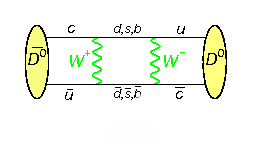
\includegraphics[scale=0.8]{figs/Deon_mixing_feyn.png}
\end{center}
\caption{\textit{Feynmann diagram showing the process by which the two $D^{0}$ states mix. This process is the only known mixing process which contain the d,s,b quarks in this position \cite{Deon_Mixing_Feyn}}}
\label{Deon_Mixing_Feyn}
\end{figure}

The first stage in detecting CPV in any system is to find mixing between a particle and its anti-particle. As in the case of Kaon and B-meson mixing we define the $CP$ eigenstates of the D meson to be linear combinations of flavour eigenstates.

\begin{equation}\label{DeonLinComb}
\ket{D^{0}_{1,2}} = p \ket{D^{0}} \pm q \ket{\bar{D}^{0}}
\end{equation}

\noindent Where for normalization $|p|^{2}+|q|^{2} = 1$. In the absence of CPV the $\ket{D_{1}}$ state is a $CP$ even state while the $\ket{D_{2}}$ state is a $CP$ odd state. As expected, we will see CPV in mixing if $|p| \neq |q|$. Clear evidence for mixing between these states was announced in 2007 and published in 2008 by the BaBar collaboration, followed shortly by the Belle collaboration \cite{BabarD0mixing}\cite{BelleD0mixing}. Results from both experiments show a small amount of $D^{0}$ mixing with 3.9 $\sigma$ certainty, at a level which is consistent with SM predictions in the order of $|x|,|y| \leq \e{-2}$, see Eqn.(\ref{xyDeonMixing}) \cite{Babar_D0_Review}. However, measured $CP$ violating parameters were consistent with zero, and thus with no CPV.

Two decays and their corresponding anti-particle decays are important for the measurement of mixing in the D meson system. The doubly Cabbibo suppressed (DCS) $D^{0} \rightarrow K^{+} \pi^{-}$ known as the wrong sign (WS) decay and $D^{0} \rightarrow K^{-} \pi^{+}$ Cabbibo favoured (CF) decay called the right sign (RS), are used. Two parameters which determine the amount of mixing in a system are defined as:

\begin{align}\label{xyDeonMixing}
x = \frac{\Delta M}{\Gamma} & & y = \frac{\Delta \Gamma}{2 \Gamma}
\end{align}

\noindent where $M= (M_{1}+M_{2})/2$ is average mass,$\Gamma = (\Gamma_{1}+\Gamma_{2})/2$ is average lifetime and $\Delta A \vcentcolon= A_{2} - A_{1}$. An approximation to the time dependence of the WS decay in the absence of CPV is given by \cite{BabarD0mixing}:

\begin{align*}
\frac{T_{WS}(t)}{e^{-\Gamma t}} & \propto R_{D} + \sqrt{R_{D}} y \Gamma t + \frac{{x'}^2 + {y'}^2}{4} (\Gamma t)^{2} \\
                             x' & = x \cos (\delta) + y \sin (\delta)\\
                             y' & = y \cos (\delta) - x \sin (\delta)
\end{align*}

\noindent Where $R_{D}$ is the ratio of the amplitudes of the DCS decay to to CF deacy and $\delta$ is the strong phase difference between the DCS and CF decays. If there is no CPV then we would expect $x' = x$ and $y' = y$. By measuring this time dependence and fitting the results to this formula, it is possible to compare predicted values of x' and y' from various theoretical models and see which best fits the data. \cref{BaBar_D0_Mixing_Results.png} shows the results of the first experiment at BaBar while \cref{LHCb_D0_Mixing_Results.png} shows more recent results from LHCb with a confidence of $5 \sigma$. Flavour tagging of the $D^{0}$ is used in these experiments. The sign of a pion known as the ``slow pion'' from the decay $D^{0*} \rightarrow D^{0} \pi^{+}_{s}$ is compared to the sign of the final product Kaon. Where $D^{0*}$ is a heavier, and thus more energetic version of the $D^{0}$ meson. If the signs are the same, the decay is WS, if they are opposite then the decay is RS. Misidentifying a random pion - not from the $D^{0*}$ decay - as the slow pion causes events which do not contain $D^{0}$ decays to be included in analysis. This creates a background which obstructs the signal data. Other sources of background are misreconstructed $D^{0}$ and combinatorial sources. Misreconstruction is due in part to semi-leptonics decays of the $D^{0}$ or $\bar{D}^{0}$ in which the detector has misidentified a lepton as a pion. Combinartorial background is caused by D mesons being produced not from $D^{0*}$, but from various possible decays of a B-meson. All of these backgrounds are reduced and excluded from the signal decays by making offline cuts to various parameters. These parameters include the the $\chi^{2}$ of the track, vertex and impact parameters of the partilces, the momentum and the mass as well as many others. Mass is plotted in two ways, the reconstructed $D^{0}$ mass distribution $(m_{K \pi})$ and the mass difference between the reconstructed $D^{0*}$ and the $D^{0}$ mass $(\Delta m)$ \cite{Kevin}. Signal events are identifed by a mass peak in the correct place in both $m_{K \pi}$ and $(\Delta m)$, random pion background has a peak in $m_{K \pi}$ but no peak in $(\Delta m)$, and vise versa for misreconstracted particles. Combinatorial background has no peak in either mass distribution. These techniques are of course universal to most particle physics experiemnts. 

\begin{figure}[h!]
\begin{center}
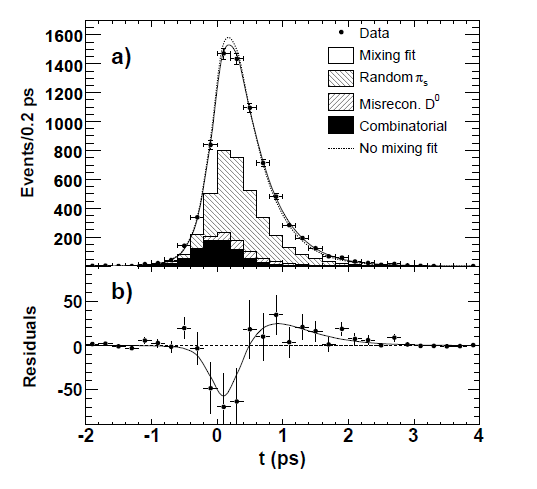
\includegraphics[scale=0.4]{figs/BaBar_D0_Mixing_Results.png}
\end{center}
\caption{\textit{Results from the first $D^{0}$ mixing experiments at BaBar, which plots the time distribution of WS decays. It is clear that the data best fits the mixing hypothesis. Backround contributions from wrongly identified $\pi^{+}_{s}$, misconstructed $D^{0}$ decays and combinatorial contributions from $D^{0}$ production from $B^{0}$ decays are removed}}
\label{BaBar_D0_Mixing_Results.png}
\end{figure}

\begin{figure}[h!]
\begin{center}
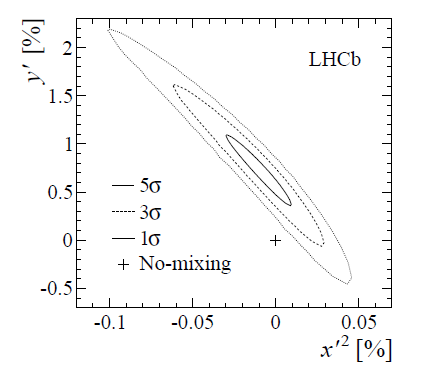
\includegraphics[scale=0.4]{figs/LHCb_D0_Mixing_Results.png}
\end{center}
\caption{\textit{2013 Results from LHCb of $D^{0}$ mixing with a confidence of $5 \sigma$. This is the first conclusive evidence for $D^{0}$ made by one experiemnt. The cross marks the no-mixing values of x' and y'}}
\label{LHCb_D0_Mixing_Results.png}
\end{figure}

CPV in mixing in this system is described by the parameter $A_{m}$ defined by:

\begin{equation*}
A_{m} = \frac{|q/p|^{2} - |p/q|^{2}}{|q/p|^{2} + |p/q|^{2}}
\end{equation*}

\noindent Where p and q are the coeffiiencts in the linear combinations (\ref{DeonLinComb}). If this value is found to not be zero then CPV in D meson mixing will be proved. Similarly for direct CPV we define:

\begin{equation*}
A_{d} = \frac{|A_{f}|^{2} - |\bar{A}_{f}|^{2}}{|A_{f}|^{2} + |\bar{A}_{f}|^{2}}
\end{equation*}

\noindent Where $A_{f}$ is the decay amplitude of $D^{0}$ to some final state f, and $\bar{A}_{f}$ is the decay amplitude of $\bar{D}^{0}$ to the state $\bar{f}$. These two parameters can be combined to construct the quantity $\lambda_{f}$ defined by \cite{LHCbAsymmetry}:

\begin{equation*}
\lambda_{f} = \frac{q \bar{A}_{f}}{p A_{f}} = - \eta_{CP} \bigg|\frac{q}{p}\bigg| \bigg|\frac{\bar{A}_{f}}{A_{f}}\bigg| e^{i \phi}
\end{equation*}

\noindent Where $\eta_{CP}$ is the $CP$ eigenvalue of the state f and $\phi$ is the phase between $q/p$ and ${\bar{A}_{f}}{A_{f}}$ and is chosen by convention so that $\ket{D_{1}}$ is an even $CP$ eigenstate. To date there has been no evidence for CPV in the D meson system. Measurements are ongoing at LHCb and if the addition of the 2013 data does not find evidence for CPV then we must wait till the restart of the LHC in 2015. The mush larger luminosity expected after the upgrade will hopefully supply the necessary statistics to conclusively measure a non-zerp value of one of the above parameters. 





